% Copyright 2009 by Tomasz Mazur
%
% This file may be distributed and/or modified in all ways.

%\documentclass[xcolor=pdftex,t,11pt]{beamer}
\documentclass[xcolor=pdftex,t,11pt,handout]{beamer}

%%%%%%%%%%%%%%%%%%%%%%%%%%%%%%%%%%
%       SET OPTIONS BELOW        %
%%%%%%%%%%%%%%%%%%%%%%%%%%%%%%%%%%
\usepackage[icelandic, english]{babel}
\usepackage{t1enc} 
\usepackage{textcomp}
\usepackage[
% Toggle showing page counter
pagecounter=true,
%
% String to be used between the current page and the
% total page count, e.g. of, /, from, etc.
pageofpages=of,
%
% Defines the shape of bullet points. Available options: circle, square
bullet=circle,
%
% Show a line below the frame title. 
titleline=true,
%
% Set the style of the title page (true for fancy, false for standard)
alternativetitlepage=true,
%
% Institution logo for fancy title page.
% Comment out to remove the logo from the title page.
% IMPORTANT: THERE IS A BUG IN SOME VERSIONS OF PDFLATEX AND FONTS
% ON THE LOGOS ARE NOT RENDERED PROPERLY. IN SUCH A CASE ADD `2` 
% TO THE NAME OF THE LOGO, E.G. comlab2 INSTEAD OF comlab
titlepagelogo=../hilogo,
%
% Department footer logo for fancy title page
% Comment out to remove the logo from the footer of the title page/
% IMPORTANT: THERE IS A BUG IN SOME VERSIONS OF PDFLATEX AND FONTS
% ON THE LOGOS ARE NOT RENDERED PROPERLY. IN SUCH A CASE ADD `2` 
% TO THE NAME OF THE LOGO, E.G. comlab2 INSTEAD OF comlab
%titlepagefooterlogo=images/titlepage/comlab,
%
% Institution/department logo for ordinary slides
% Comment this line out to remove the logo from all the pages.
% Available logos are: ou, comlab, comlabinline, comlabou
% IMPORTANT: THERE IS A BUG IN SOME VERSIONS OF PDFLATEX AND FONTS
% ON THE LOGOS ARE NOT RENDERED PROPERLY. IN SUCH A CASE ADD `2` 
% TO THE NAME OF THE LOGO, E.G. comlab2 INSTEAD OF comlab
ordinarypageslogo=../hilogoname,
%
%
% Add watermark in the bottom right corner
%watermark=<filename>,
%
% Set the height of the watermark.
%watermarkheight=100pt,
%
% The watermark image is 4 times bigger than watermarkheight.
%watermarkheightmult=4,
]{../beamerThemeTorino} 

% Select color theme. Available options are:
% mininmal, greenandblue, blue, red
%\usecolortheme{hi}
\usepackage{../beamercolorthemehi}

%Select different font themes.Available options are:
% default, serif, structurebold, structureitalicserif, structuresmallcapsserif
\usefonttheme{structurebold}

\setbeamercovered{transparent}
\usepackage{tabularx}

\usepackage{natbib} %citep and citet
%\bibpunct[:]{(}{)}{;}{a}{}{,}
%\renewcommand{\bibsection}{\subsubsection*{\bibname } }

\newcommand{\bi}{\begin{itemize}\item}
\newcommand{\ei}{\end{itemize}}

\usepackage{latexsym}
\usepackage{amsmath,bm,amssymb}

\usepackage[colorinlistoftodos]{todonotes}
\usepackage{comment}
\usepackage{multirow}
\usepackage{rotating}
\usepackage{longtable}
\usepackage{paralist}
\usepackage[perpage,symbol*]{footmisc}
\usepackage{tabu}
\usepackage{tabularx}
\newcommand{\tcr}[1]{{\color{red} #1}}
\newcommand{\tcb}[1]{{\color{blue} #1}}
\newcommand{\tcg}[1]{{\color{green} #1}}

\usepackage{paralist}


%\renewcommand{\rho}{{\varrho}}

\renewcommand{\vec}[1]{\mathbf{#1}}
\newcommand{\vphi}{{\boldsymbol{\phi}}}
\newcommand{\Exp}{{\mathbb E}}
\newcommand{\inner}[2]{\big<{#1}\cdot{#2}\big>}
\newcommand{\norm}[1]{\lVert#1\rVert}

\newcommand{\vsigma}{{\vec{\sigma}}}
\newcommand{\mat}[1]{\mathbf{#1}}
\newcommand{\R}{{\mathbb R}}
\newcommand{\strng}[1]{{\mbox{\tt #1}}}
\newcommand{\abs}[1]{\lvert#1\rvert}
\newcommand{\argmax}{\mathop{\rm argmax}}
\newcommand{\argmin}{\mathop{\rm argmin}}


\hyphenpenalty=750
\hyphenation{heur-ist-ics}
\hyphenation{algo-rithm}

% job-related
\newcommand{\phiproc}{$\phi_1$}
\newcommand{\phistartTime}{$\phi_2$}
\newcommand{\phiendTime}{$\phi_3$}
\newcommand{\phiwrmJob}{$\phi_4$}
\newcommand{\phiwait}{$\phi_5$}
\newcommand{\phiarrivalTime}{$\phi_6$}
\newcommand{\phijobOps}{$\phi_7$}
% mac-related
\newcommand{\phimac}{$\phi_8$}
\newcommand{\phimacFree}{$\phi_9$}
\newcommand{\phiwrmMac}{$\phi_{10}$}
\newcommand{\phimacOps}{$\phi_{11}$}
% flow-related
\newcommand{\phislotCreated}{$\phi_{12}$}
\newcommand{\phislotReduced}{$\phi_{13}$}
\newcommand{\phislots}{$\phi_{14}$}
\newcommand{\phislotsTotal}{$\phi_{15}$}
% schedule related
\newcommand{\phimakespan}{$\phi_{16}$}
\newcommand{\phiwrmTotal}{$\phi_{17}$}
\newcommand{\phitotProc}{$\phi_{18}$}
\newcommand{\phistep}{$\phi_{19}$}
% global
\newcommand{\phiMWR}{$\phi_{20}$}
\newcommand{\phiLWR}{$\phi_{21}$}
\newcommand{\phiSPT}{$\phi_{22}$}
\newcommand{\phiLPT}{$\phi_{23}$}
\newcommand{\phiRND}{$\phi_{24}$}


\usepackage{cleveref} % must come last! 
 % put your own shorthand declarations in this document
%%%%%%%%%%%%%%%%%%%%%%%%%%%%%%%%%%
%       PRESENTATION INFO        %
%%%%%%%%%%%%%%%%%%%%%%%%%%%%%%%%%%

\author{Helga Ingimundard\'{o}ttir\\Thomas Philip R\'{u}narsson}
\title{Data Driven Design of Blended Dispatching Rules}
\subtitle{Using Preference Learning and Evolutionary Search\newline Case study for JSP and PFSP}
\institute{University of Iceland}	
\date{September 13$^{th}$, 2013}


\begin{document}

%%%%%%%%%%%%%%%%%%%%%%%%%%%%%%%%%%
%       SLIDE DEFINITIONS        %
%%%%%%%%%%%%%%%%%%%%%%%%%%%%%%%%%%

\begin{frame}[plain]
	\titlepage
\end{frame}

\frame{
\frametitle{Outline}
\tableofcontents[part=0] % part=0, sectionstyle=show/shaded
}

\section{Introduction}
\frame{\tableofcontents[currentsection]}

\frame{
\frametitle{Motivation}

\begin{block}{General Goal}
\begin{itemize} 
\item General goal is how to search for \emph{good} solutions for an arbitrary problem domain. 
\item Automate the design of optimization algorithms. 
\item Use of randomly sampled problem instances and their corresponding optimal vs. suboptimal solutions.
\end{itemize}
\end{block}
}

\frame{\frametitle{Case Study: JSP and PFSP}
\begin{block}{Abstract}
\begin{itemize}
\item Framework for creating dispatching rules for JSP and PFSP.
\item Supervised learning based on optimal and sub-optimal solutions. 
\item Training data is randomly generated problem instances and their optimal solutions. Method is purely \alert{data-driven}.
\item \alert{Linear classification} to identify good dispatches from worse ones.
\item \alert{Robust} for higher dimensions. 
\end{itemize}
\end{block}
\textbf{Keywords:} Scheduling $\bullet$ Composite dispatching rules $\bullet$ JSP  $\bullet$ PFSP $\bullet$ Generating training data $\bullet$ Sampling $\bullet$ Ranking $\bullet$ Scalability $\bullet$ Ordinial Regression $\bullet$ Evolutionary Search
}


\section{Job Shop Scheduling}
\frame{\tableofcontents[currentsection]}

\frame[allowframebreaks]{
\frametitle{Job Shop Scheduling}
\begin{block}{JSP}
	Simple job shop scheduling problem  is where $n$ jobs are scheduled on a set of $m$ machines, subject to constraints:
	\begin{itemize}
	\item each job must follow a predefined machine order,
	\item that a machine can handle at most one job at a time.
	\end{itemize}
	
	\textbf{Objective:} schedule the jobs so as to minimize the maximum completion time, i.e. makespan, $C_{\max}$.
\end{block}
\begin{block}{PFSP}	
    Permutation flow shop scheduling is the same as JSP except the predefined machine order is homogeneous for all jobs.	
\end{block}
%\begin{itemize}
%	\item Job $j$ has an indivisible operation time on machine $a$, $p(j,a)$, which is assumed to be integral, where $j \in\{1,..,n\}$ and $a\in\{ 1,..,m\}$. 
%	\item Job $j$ has a specified processing order through the machines, it is a permutation vector, $\sigma_j$, of $\{1,..,m\}$, i.e. $j$ can be processed on $\sigma_j(a)$ only after it has completed on $\sigma_j(a-1)$.
%	\begin{itemize} \item Permutation flow shop scheduling (PFSP) is when $\sigma_j$ is fixed $\forall j$. \end{itemize}
%\end{itemize}
\begin{block}{Problem space distributions used in experimental studies}
\begin{table}\centering
{\scriptsize \renewcommand{\arraystretch}{0.6}
\begin{tabular}{|l|l|c|c|c|l|}\hline 
type&name&size ($n\times m$)& $N_{\text{train}}$&$N_{\text{test}}$  & note 
\\ \hline\hline 
\multirow{4}{*}{JSP}
&$\mathcal{P}_{jrnd}^{6\times5}$ & $6\times5$ & 500 & 500 & random \\
&$\mathcal{P}_{jrndn}^{6\times5}$ & $6\times5$ & 500 & 500 & random-narrow \\
&$\mathcal{P}_{jrnd}^{10\times10}$ &$10\times10$& -- & 500 & random \\
&$\mathcal{P}_{jrndn}^{10\times10}$ &$10\times10$& -- & 500 & random-narrow \\ \hline\hline 
\multirow{6}{*}{PFSP}
&$\mathcal{P}_{frnd}^{6\times5}$ &$6\times5$& 500&500& random \\ 
&$\mathcal{P}_{frndn}^{6\times5}$&$6\times5$& 500&500& random-narrow \\ 
&$\mathcal{P}_{fjc}^{6\times5}$  &$6\times5$& 500&500& job-correlated \\ 
&$\mathcal{P}_{frnd}^{10\times10}$ &$10\times10$&--&500&random \\ 
&$\mathcal{P}_{frndn}^{10\times10}$&$10\times10$&--&500& random-narrow \\ 
&$\mathcal{P}_{fjc}^{10\times10}$  &$10\times10$&--&500& job-correlated \\ 
\hline
\end{tabular}
}
\end{table}

\end{block}
\framebreak
\begin{block}{Simple Priority Dispathcing Rules}
\begin{figure} \centering 
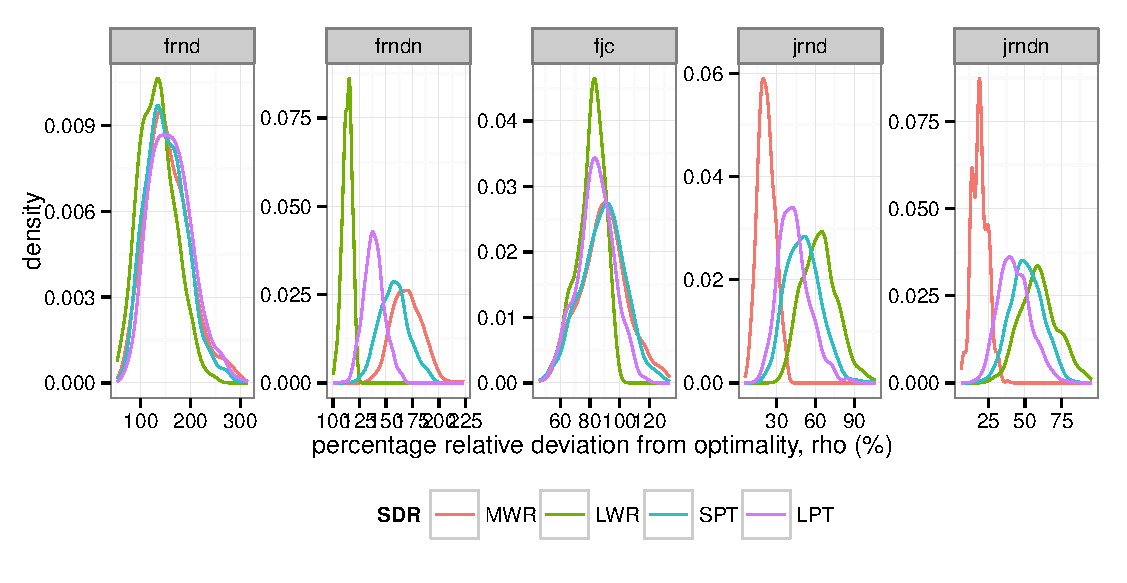
\includegraphics[width=0.8\textwidth]{figures/SDR10x10color}
\end{figure}
\end{block}

\begin{block}{Dispatching rules (DR) for constructing JSSP}
\begin{itemize}
	\item Starts with an empty schedule and adds on one job at a time. 
	\item When a machine is free the DR inspects the waiting/available jobs and selects the job with the \alert{highest priority}. 
	\item Complete schedule consists of $\ell=n\times m$ sequential dispatches.
	\item At each dispatch $k$ features $\vphi(k)$ for the temporal schedule are calculated.
	\item Performance of DR is compared with its optimal makespan, as percentage relative deviation from optimality: $\rho=\frac{C_{\max}^{DR}-C_{\max}^{opt}}{C_{\max}^{opt}}\cdot 100\%$
\end{itemize}
\end{block}

\begin{block}{Features for JSSP}
\begin{table}[t!]
 {\scriptsize
 \begin{center}
  \begin{tabular}{|c|l|}
   \hline\hline
  $\vphi$ & Feature description \\ \hline
  $\phi_1$ & processing time for job on machine\\
  $\phi_2$ & start-time \\
  $\phi_3$ & end-time \\
  $\phi_4$ & when machine is next free \\
  $\phi_5$ & current makespan \\
  $\phi_6$ & work remaining \\
  $\phi_7$ & most work remaining \\
  $\phi_8$ & slack time for this particular machine \\
  $\phi_9$ & slack time for all machines \\
  $\phi_{10}$ & slack time weighted w.r.t. number of operations already assigned \\
  $\phi_{11}$ & time job had to wait\\
  $\phi_{12}$ & size of slot created by assignment \\
  $\phi_{13}$ & total processing time for job \\
 \hline\hline
  \end{tabular}
 \end{center}}
\end{table}
\end{block}
}

\frame{
\frametitle{Job Shop Scheduling}
\begin{example}
	\begin{center}
		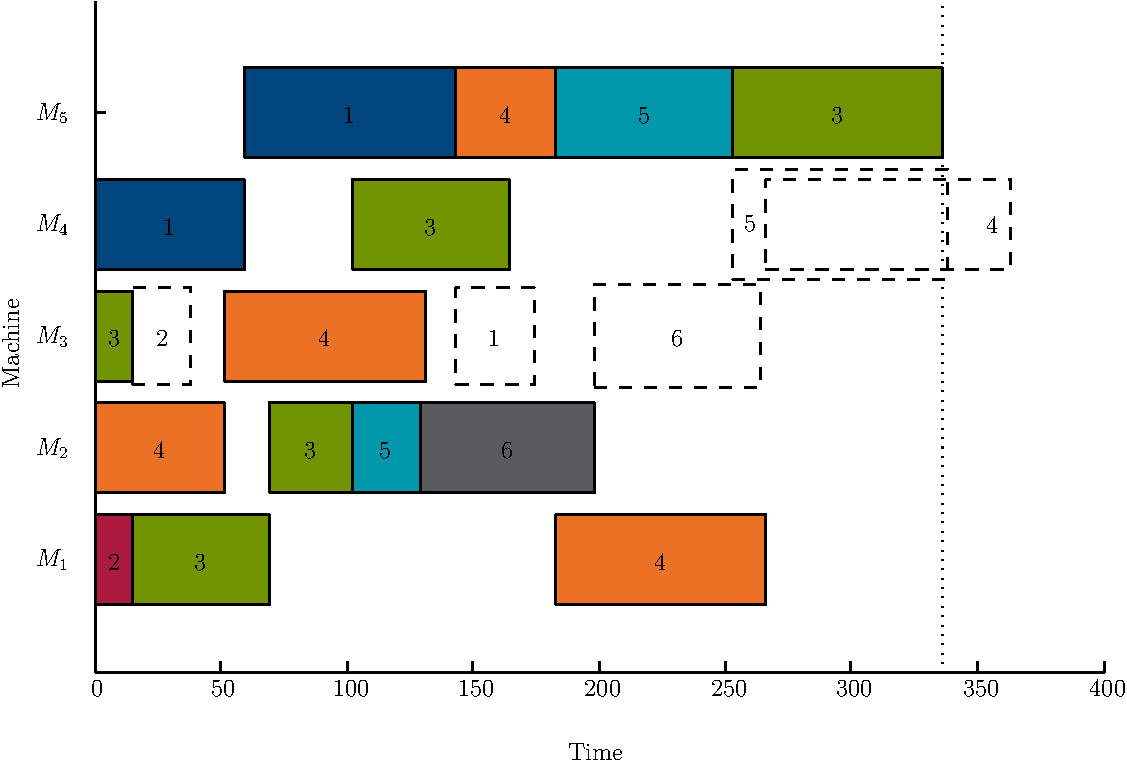
\includegraphics[width=0.5\columnwidth]{figures/jssp_example}
	\end{center}
	A schedule being built at step $k=16$. The dashed boxes represent five different possible jobs that could be scheduled next using a DR.
\end{example}
}

\section{Preference models}
\frame{\tableofcontents[currentsection]}

\frame[allowframebreaks]{\frametitle{Ordinal Regression}
\begin{block}{Preference learning problem}
Specified by a set of \alert{preference pairs}:
\begin{equation*}
S = \left\{\left\{\vec{z}_o,+1)\right\}_{k=1}^{\ell},\left\{\vec{z}_s,-1)\right\}_{k=1}^{\ell}
\;|\;\forall o\in \mathcal{O}^{(k)},s\in \mathcal{S}^{(k)}
\right\}\subset \Phi\times Y \label{eq:S}
\end{equation*}
where the set of point/rank pairs are:
\bi Optimal decision: $\vec{z_o}=\vphi^{(o)}-\vphi^{(s)}$, ranked $+1$
\item Sub-optimal decision: $\vec{z_s}=\vphi^{(s)}-\vphi^{(o)}$, ranked $-1$
\ei
\end{block}
\framebreak

\bi Mapping of points to ranks: $ \{h(\cdot) : \Phi \mapsto Y\}$ where 
\begin{equation}
\vphi_o \succ \vphi_s \quad \Leftrightarrow \quad h(\vphi_o) > h(\vphi_s) \nonumber
\end{equation}

\item The preference is defined by a linear function, i.e. \alert{PREF model}:
$$ h(\vphi) = \sum_{i=1}^d w_i \vphi = \inner{w}{\phi}. $$
\item Logistic regression learns the optimal parameters $\vec{w}$ by solving:
$$ \min_{\vec{w}}\quad \tfrac{1}{2}\inner{w}{w} + C \sum_{j=1}^{\abs{S}} \log\left(1 + e^{-y_j \inner{w}{z_j}}\right) $$ 
\ei

}

\frame[allowframebreaks]{\frametitle{Generating prefernce set $S$}
\begin{block}{A seperate DR for each dispatch iteration}
\bi At each dispatch  $k$ a number of data pairs are created
	\bi for each of the $N_{\text{train}}$ problem instance created. \ei 
	\item Deliberately create a separate data set for each dispatch  
	\bi Resulting in $\ell$ linear scheduling rules for solving a $n \times m$ JSSP. \ei
\ei 
\end{block}
Defining the size of the training set as $l=\abs{\Phi}$, gives the size of the preference set as $\abs{S}=2l$. 
\bi If $l$ is too large, than sampling needs to be done. \ei 

\begin{block}{Previous sampling approach  }
The strategy was to follow some \alert{single optimal job} $j\in\mathcal{O}^{(k)}$, thus creating $\abs{\mathcal{O}^{(k)}}\cdot\abs{\mathcal{S}^{(k)}}$ feature pairs at each dispatch $k$, resulting in a training size of: 
\begin{equation}
l = \sum_{q=1}^{N_{\text{train}}}\left(\sum_{k=1}^\ell \abs{\mathcal{O}^{(k)}}\cdot\abs{\mathcal{S}^{(k)}}\right) \nonumber
\end{equation}
\end{block}
For the data distribution considered there, this simple sampling was sufficient for a favourable outcome. However for a considerably harder data distribution this strategy did not work well.

% \begin{quote} Motivation: a brute force approach to investigate the feasibility of finding optimal weights $\vec{w}$.\end{quote} 
\framebreak
\begin{block}{Trajectory sampling strategies explored for $S$,}
\begin{description}
\item[$S^{opt}$] follow some (random) optimal task
\item[$S^{cma}$] follow the task corresponding to highest priority, computed with fixed weights $\vec{w}$, which were obtained by optimising with CMA-ES. 
\item[$S^{mwr}$] follow the SDR most work remaining (MWR).
\item[$S^{lwr}$] similar to $S^{mwr}$ except for least work remaining (LWR).
\item[$S^{all}$] union of all of the above.
\end{description}
\end{block}

\framebreak
\begin{block}{Ranking strategies explored for $S$,}
\begin{description}
\item[$S_{b}$] all optimum rankings $r_1$ versus all possible sub-optimum rankings $r_i, i\in\{2,...,n'\}$, preference pairs added.
\item[$S_{f}$] full subsequent rankings, i.e. all possible combinations of $r_i$ and $r_{i+1}$ for $i\in\{2,...,n'\}$, preference pairs added.
\item[$S_{p}$] partial subsequent rankings, i.e. sufficient set of combinations of $r_i$ and $r_{i+1}$ for $i\in\{2,...,n'\}$, preference pairs added. Note that $S_{p}\subset S_{f}$.
\item[$S_{all}$] union of all of the above.
\end{description}
where $r_1>r_2>...>r_{n'} (n'<n)$ are the rankings of the ready-list at each time step.
\end{block}
}

\section{Evolutionary search with CMA-ES}
\frame{\tableofcontents[currentsection]}

\frame{\frametitle{Evolutionary search}
Instead of using logistic regression for to find the weights $\vec{w}$ for linear preference function:
$$ h(\vphi) = \sum_{i=1}^d w_i \vphi = \inner{w}{\phi}. $$
a widely-used evolutionary algorithm, Covariance Matrix Adaptation Evolution Strategy (\alert{CMA-ES}), is applied to directly minimise the expected relative error, i.e. \alert{$\mathbb{E}\left[\rho\right]$} (note, could also minimise $\mathbb{E}\left[C_{\max}\right]$)

\begin{description}\item[Benefit] No need to collect preference set $S$
\item[Drawback] Computationally expensive to evaluate $\mathbb{E}\left[\rho\right]$
\end{description}

}



\section{Experiments}
\frame{\tableofcontents[currentsection]}

\frame[allowframebreaks]{\frametitle{Experiments}
\begin{block}{Size of preference set $S$ for $\mathcal{P}_{jrnd}^{6\times5}$}
\begin{figure} \centering
%\includegraphics[width=0.3\textwidth]{figures/tmp/sizeS_opt_p1-eps-converted-to.pdf}
%\includegraphics[width=0.3\textwidth]{figures/tmp/sizeS_CMA_p1-eps-converted-to.pdf}
%\includegraphics[width=0.3\textwidth]{figures/tmp/sizeS_MWR_p1-eps-converted-to.pdf}
%\\\hfill$S^{opt}$\hfill$S^{cma}$\hfill$S^{mrw}$
\end{figure}
$S_{b}$ in blue, $S_{f}$ in red and $S_{p}$ in green.
\end{block}
\framebreak
\begin{block}{Size of preference set $S_{p}$}
\begin{figure} \centering
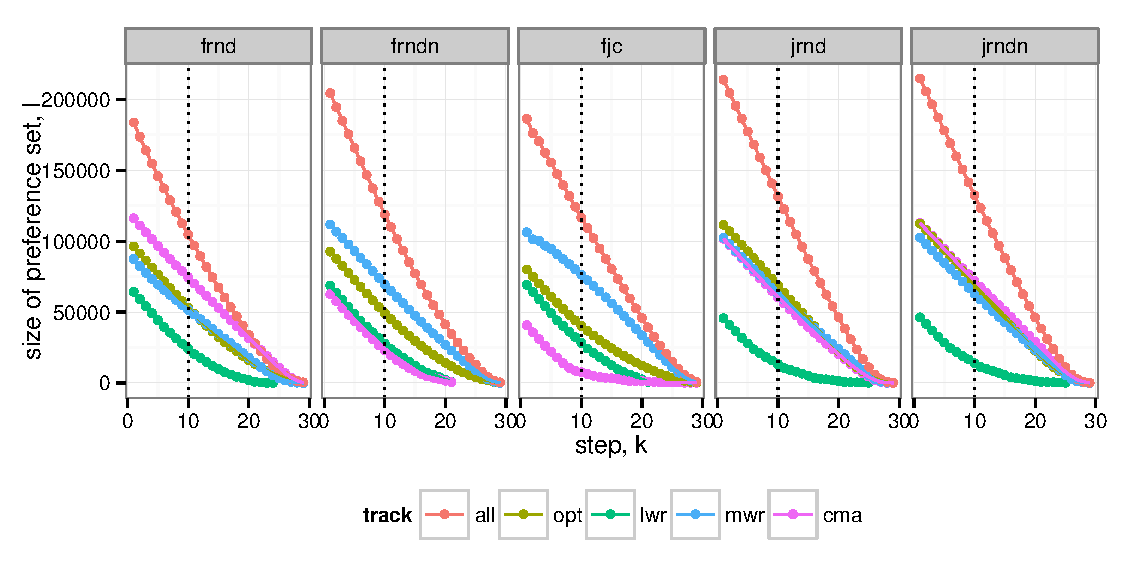
\includegraphics[width=0.8\textwidth]{figures/NUMtrinstances_d30color}
\end{figure}
\end{block}
\framebreak
\begin{block}{Linear PREF models and CMA-ES obtained weights}
\begin{figure} \centering
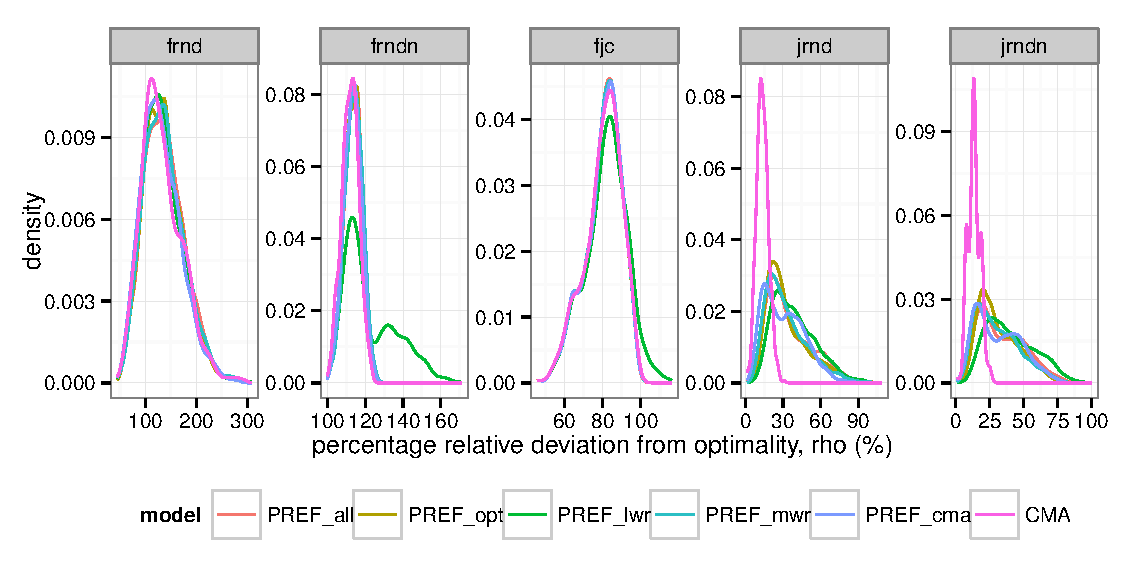
\includegraphics[width=0.8\textwidth]{figures/10x10tested4trainset}
\end{figure}
\end{block}
}

\section{Summary and conclusions}
\frame{\tableofcontents[currentsection]}

\frame[allowframebreaks]{\frametitle{Summary and conclusions}

\bi Introduced a framework for learning linear composite dispatch rules for scheduling. 
\item The approaches find linear weights by either \alert{direct optimisation with CMA-ES} or via \alert{preference learning} by collecting preference pairs whilst sampling the state space of the schedule strategically. 
\ei
\begin{block}{CMA-ES optimisation}
Benefits: 
\bi Does not rely on optimal solutions
\item Scalable
\ei 
Drawbacks:
\bi Computationally expensive .
\item Limited to linear preference function $h(\cdot)$
\ei 
Future Work:
\bi Mediate evolutionary search by use of surrogate models which indirectly estimate mean expected error w.r.t. current population without a loss in performance
\ei 
\end{block}
\begin{block}{PREF models}
Benefits:
\bi Scalable 
\item Robust to different data distributions
\ei
Drawbacks:
\bi Must know the optimal solution of the problem a priori to correctly classify optimal decisions from suboptimal ones
\ei 
Future work:
\bi Adaptable to non-linear preferences function, i.e. project the feature space onto a higher dimension thereby updating $h(\cdot)$ to a kernel based function which should yield lower expected $C_{\max}$ 
\ei 
\end{block}

}
\frame{
\frametitle{Thank you for your attention}
\vspace{2cm}
\begin{center} \pause {\huge\bf Questions?} \end{center}
\vfill
\begin{flushright} Helga Ingimundard\'{o}ttir, \url{hei2@hi.is}\end{flushright}
}
\frame[allowframebreaks]{\frametitle{References}
\bibliographystyle{abbrv} 
{\footnotesize % http://www.csc.liv.ac.uk/research/local/grants/

\documentclass[12pt,a4paper]{article}

%\usepackage[latin1]{inputenc}
%\usepackage[T1]{fontenc}

\usepackage{setspace}
\usepackage{lastpage}
\usepackage{fancyhdr}
\usepackage{hyperref}
%\renewcommand{\rmdefault}{phv}\renewcommand{\sfdefault}{phv}
%\usepackage[landscape]{geometry}
\usepackage{amsmath,pgf,tikz}
\usepackage{amsfonts}
\usepackage{amssymb}
%\addtolength{\textwidth}{1cm}
%\setlength{\topmargin}{-2cm}
%\addtolength{\oddsidemargin}{-.5cm}
%\addtolength{\evensidemargin}{-.5cm}
\renewcommand{\vec}[1]{\mathbf{#1}}

\addtocounter{page}{-1}

\renewcommand{\refname}{\normalsize References} % Using "Sources" as the title of the section

\newcounter{rownum}
% \timeline{tick}
\newcommand*{\timeline}[1]{    % vertical timeline
  \draw (t_cur) ++(1,0) node[fill=white,coordinate] (t_cur) {#1};
}

% \barshape{value}{length}{color}{opacity}
\newcommand*{\barshape}[4]{
  \draw[fill=#3,opacity=#4] (t_cur) -- ++(0,.3) -- ++(#2,0) -- ++(0, -.3) -- ++(0,-.3) -- ++(0-#2,0) -- cycle;
  \path (t_cur) -- node {#1} ++(#2,0) node[coordinate] (t_cur) {};
}

% \lagtime{value}{length}
\newcommand*{\lagtime}[2]{
    \barshape{#1}{#2}{white}{0}
}

% \activity{value}{length}
\newcommand*{\activity}[2]{
    \barshape{\small{#1}}{#2}{black!50}{1}
}

% \activityrow{name}
\newcommand{\activityrow}[1]{
  \path (0,\value{rownum}) node[left] {\small{#1}} node[coordinate] (t_cur) {};
  \addtocounter{rownum}{-1}
}

% \begin{gantt}[timeline_name]{num_of_cols}{num_of_rows}
\newenvironment{gantt}[3][]{
  \begin{tikzpicture}[draw=black, yscale=.7,xscale=1]
    \draw (0,.5) rectangle (#2+1,-#3+.4);
    \setlength{\unitlength}{1cm}
    \setcounter{rownum}{0}
    \activityrow{#1}                % number of horizontal rows
    % -- horizontal time slice lines
%    \foreach \t in {1,...,#2}{
    \foreach \t in {jan$^{'12}$,apr-,jul-,oct-,jan$^{'13}$,apr-,jul-,oct-,jan$^{'14}$,apr-,jul-,oct-}{
      \timeline{\t}
      \draw[dotted] (t_cur) +(0,.4) node[fill=white, anchor=north] {\t} -- ++(0,.4-#3);
    }
}{\end{tikzpicture}}


%\author{T\'omas Philip R\'unarsson}
%\title{Data Driven Design\\ of Fast Approximate Algorithms}
\title{\large T\'omas Philip R\'unarsson \\ \ \\ \ \\ }
\author{\LARGE Data Driven Design\\ \LARGE of Fast Approximate Algorithms\\ \ \\ \ \\}
\date{The Icelandic Research Fund 2014\\
Project Grant - New proposal\\
Appendix A (Detailed project description)\\
\ \\ 
\ \\
\normalsize Reykjav\'ik, 3/6/2013}

\lhead{The Icelandic Research Fund 2014\\ Detailed project description}
\chead{}
\rhead{T\'omas Philip R\'unarsson\\}
\lfoot{Project Grant\\ New proposal}
\cfoot{}
\rfoot{Data Driven Design of Algorithms \\ Page \thepage \ of \pageref{LastPage}}
\renewcommand{\headrulewidth}{0.4pt}
\renewcommand{\footrulewidth}{0.4pt}

\begin{document}
\maketitle
\pagestyle{fancy}
\thispagestyle{empty}


\newpage
\onehalfspacing

\section*{\normalsize a.) State of the art and proficiency}

Designing algorithms to solve problems approximately, for tasks that cannot be solved exactly, is a time consuming 
trial and error process requiring problem specific insights. The alternative to hand-crafting heuristics, is a data 
driven approach to automate, in part, this design process. Typically this data consists of numerous problem instances 
and when possible their exact solution. The first successful application of this idea was presented by Minton 
back in 1996 \cite{minton1996automatically}. There the idea was to automatically design problem specific versions of 
constraint satisfaction algorithms. Using data generated from different instance distributions programs were designed 
that were on par with hand-crafted programs. 

Depending on the underlying data distribution of problem instances, different heuristic perform differently. This 
is due to the fact that any algorithm which has superior performance in one class of problems is inevitably inferior 
over another class, c.f. the \emph{no free lunch} theorems \cite{Wolpert97nofree}. 
%  number of ?no free lunch? (NFL) theorems are presented which establish that for any algorithm, any elevated 
%performance over one class of problems is offset by performance over another class. 
The success of a heuristic is how it manages to deal with and manipulate the characteristics of its given problem 
instance. An attempt to understand the heuristic's performance is to look at the relationship between problem 
structure and heuristic effectiveness. Attempt to classify heuristic performance over instance space have been termed 
\lq\lq landmarking\rq\rq\ or \lq\lq footprints\rq\rq\ in instance space \cite{Corne10,Pfahringer00}. These studies 
involve clustering problem instances using problem specific features. As an example, a recent study shows that a 
linear combination of features for bin packing problems are related to heuristic performance \cite{Camacho2013}. In 
this study principle component analysis is used to perform the cluster analysis.
In the scope of scheduling this has been explored by the authors for jobshop scheduling by~\cite{InRu12a} and 
timetable scheduling \cite{SmithMilesLion5,Smith-Miles2012a}. Clustering with self-organizing maps indicates that 
real-world timetable problems can have a very different underlying parameter distribution that synthetically generated 
instances \cite{SmithMilesLion5}. This has also been observed in scheduling \cite{Whitley}.

Exact solutions can in some cases demonstrate how an optimal solution to a problem instance may be constructed. 
Building solutions, however, requires problem specific assignments which must be predefined for any problem type. For 
example, in bin packing this would be to assign an item to a bin and similarly for scheduling assigning a job to a 
machine. Typically, one would design assignments that guarantee the construction of legal solutions. For example, we 
would not assign an item to a full bin, or a job to a busy machine. Improvement or local search operators would 
also require the design of problem specific \lq\lq assignments\rq\rq. Deciding on an assignment requires a policy and 
it is this decision policy we aim to design and learn. In some cases the number of possible assignments is very large 
or a complex procedure is needed to create legal assignments. The common practice then is to design a number of 
problem specific procedures or heuristic for this purpose. An example of such a heuristic for the packing of a large 
number of items would be to assign the smallest one to a particular bin. The policy for selecting among these 
different assignment heuristics is now the learning problem. The most common approach to representing policies is 
through utility functions and simple one step look-ahead procedures. In this case all possible assignments or 
heuristics used for this purpose are performed and the partial solutions evaluated by the utility function. The 
assignment resulting in the highest utility is then the one chosen.  Using genetic programming this approach has been 
quite successful for bin-packing problems \cite{poli2007histogram,burke2012automating}. In some sense we can think of 
this as a classification problem where we must determine which partial solution should be selected. From this 
perspective the utility function corresponds to a classification function. The alternative to performing a look-ahead 
would be to associate the current partial solution to a particular assignment or assignment heuristic. This would seem 
to be a harder problem to solve, but a few examples of this approach exist for the design of heuristics. For example, 
in \cite{fukunaga2008automated,bader2009evolving} a genetic program, with a tree like structure, inputs properties of 
the current partial solution and all leaf nodes correspond to some predefined assignment heuristic. 

The idea of using algorithms to automatically design or tune search algorithms using hyper-heuristics was prosed in   
\cite{burke2003hyper}. The hyper-heuristic framework presented operates at a high level of abstraction and often has 
no knowledge of the domain. Typically an evolutionary algorithm will be applied to search the policy space directly. 
In this case the exact solution to generated problem instances need not be know in advance. The evolutionary 
algorithm simply searches for policies that perform on average the best over the set of training problem instances.

In~\cite{Siggi05} data is generated from a known heuristic, for job-shop scheduling, and a decision tree used to 
rediscover the heuristic from the data. However, such a technique is unable to outperform the heuristic that generated 
the training data used. This drawback was confronted in~\cite{Malik08,Russell09,Siggi10} by using data generated from 
an optimal scheduler, computed off-line.  Preferring simple to complex models, the resulting dispatching rules gave 
significantly better schedules than using popular heuristics in that field, and a lower worst-case factor from 
optimality. A similar approach is taken for timetable scheduling in~\cite{Burke06}, using case based reasoning. 
Training data is guided by the two best heuristics for timetable scheduling. The authors point out that in order for 
their framework to be successful, problem features need to be sufficiently explanatory and training data need to be 
selected carefully so they can suggest the appropriate solution for a specific range of new cases. 


Using the hype-heuristic framework HyFlex \cite{ochoa2012hyflex}.


A good overview on hyper-heuristics may be found in \cite{burke2010hyper}.


{\underline the reinforcement learning approach, Zhang and Runarsson}
\cite{Kalyanakrishnan2011} point out that meta learning can be very fruitful in reinforcement learning, and in their 
experiments they discovered some key discriminants between competing algorithms for their particular problem 
instances, which provided them with a hybrid algorithm which combines the strengths of the algorithms.


{\underline Monte Carlo approach, Runarsson x2}


Missing items:
\begin{itemize}
\item Surrogate models.
\item Handling large volumed of training data.
\item ... other ...

\end{itemize}



\section*{\normalsize b.) Objectives of the project and originality}

Things not yet done in the literature:
\begin{itemize}
\item Optimizing for speed and accuracy, dual-objective problem.
\item Design of experiment: how to sample of training data to achieve the goal of automatically generating algorithms, 
often just generated in an ad-hoc manner.
\item 
\end{itemize}

How can you speed up an algorithm? What can the data be used for within the design procedure? Data can be used for 
modelling objectives, but also for the design og heuristics to create solutions, and?


The broad objective of this research programme is to deepen our
understanding of how data may be applied to the design of fast and
approximate algorithms. 



To achieve this goal we have put together a research 
team with expertise in statistics, computing and computational intelligence. 
There are in principle three main aspects which we For this we believe a diverse set of applications 
will help tease out common ... in ...


\begin{enumerate}
\item {\bf Data generation}: to understand the properties and characteristics of the data needed to design efficient 
and effective algorithms. We will try to achieve this objective by looking at specific sub-goals. They are:
\begin{enumerate}
\item {\bf Problem instance generator}: developing numerous new problem instances from a few examples, understand to 
what extend one can expect the algorithm designed can generalize beyond these instance distributions. When many 
examples exist, as is the case in our real world problem tackled by this project, how and which instances are 
sufficient to design our algorithms.
\item {\bf Sampling}: within each instance a large amount of data may be generated. The data may be generated from 
optimal as well as 
suboptimal solutions to the instance. sub-sampling this space is also an issue. and data sampling within a problem 
instance.
\end{enumerate}
\item {\bf Parallel computing framework}: Develop a generic framework for the development of data driven designed 
algorithms. Implement numerous machine learning for large data sets on a parallel framework. 
\item {\bf Applications}: a diverse set of applications will be applied using the parallel framework, they can be put 
into two different categories:
\begin{enumerate}
\item {Designing heuristics}:
\item {Approximating objectives}:
\end{enumerate}
In each case their one data driven design will be based on read world data, whereas the second will be based on 
theoretically derived data.
\end{enumerate}


\section*{\normalsize c.) Methodology, work plan and timescale}

At the University of Iceland the following personnel will be working on the project: .... , Communication with 
external collaborators will be conducted through short visits, meetings at 
conferences, e-mail and phone.

\subsubsection*{Work-Package 1 -- Instance generation and data sampling}
\noindent {\bf Responsibility:} T. P. R\'unarsson, B. Hrafnkelsson, and PhD student.\\
%\noindent {\bf External Collaborators:} Darrell Whitley.\\
\noindent {\bf Time-frame:} 01.01.14--31.12.14.\\
\noindent {\bf Milestones:} Framework for generating problem instances and sampling training data.


\subsubsection*{Work-Package 2 -- Computational framework}

\noindent {\bf Responsibility:} T. P. R\'unarsson, Morris Riedel and PhD student.\\
%\noindent {\bf External Collaborators:} Darrell Whitley.\\
\noindent {\bf Time-frame:} 01.01.14--31.12.14.\\
\noindent {\bf Milestones:} High performance computing framework for data driven design of algorithms.


\subsubsection*{Work-Package 3 -- Fast approximate algorithms for streaming computing (STC)}
\noindent {\bf Responsibility:} P. Melsted, MSc student\\
\noindent {\bf Time-frame:} 01.01.14--31.12.14.\\
\noindent {\bf Milestones:} .

{\bf Missing description}


\subsubsection*{Work-Package 4 -- Two dimensional free form bin packing}
\noindent {\bf Responsibility:} H. Ingimundard�ttir, MSc student\\
\noindent {\bf Time-frame:} 01.01.14--31.12.14.\\
\noindent {\bf Milestones:} .

Valka ehf. is currently working on intelligent portioning solutions for fish. Current solutions are constrained to 
either fixed weights or fixed shape, and the machinery is generally  inspecting only one scheme at a time. However the 
diversity of fish within a catch can be quite varying (both respect to weight, size, and quality) and thus it would be 
appropriate to have a self-adapting algorithm that implements the best cutting pattern per fish fillet based on its 
X-Ray imagery. Moreover, the algorithm should be able to report whether gaping (�. los) is present for quality control 
purposes. 
 
It is possible to interpret the fish portioning as two-dimensional free-form bin packing problem (2D-FBP), where 
approximately rectangular portions are being cut from irregular shape, e.g. fish fillet. Unfortunately, 2D-FBP is 
generally put forth as ir/regular shapes cut from regular shapes (not vice versa). Portioning combines several 
combinations of traditional bin-packing, namely, 
\begin{itemize}
\item  trim-loss: determination of cutting pattern to minimize waste
\item         assortment: determination of ?best? fillet for cutting predefined portions in order to minimise number 
of fillets needed to fulfil an order
\item         knapsack: determination of ?best? portion for cutting, since each portion has a value based on market 
demand 
making the portioning problem a multi-objective optimization problem subject to some technical constraints, such as, 
\item         material properties: tail portions can only be taken from tail region, etc.
\item         cutting processes: a minimum distance between portions is required or order not to damage to cutters
\item         serious time constraints: the algorithm has to report the cutting paths before the fillet is situated 
near the water cutters
 \end{itemize}
The project can be divided into the following subtasks:
\begin{itemize}
\item         Literature study and establishment of the state of the art involving cutting stock problems of irregular 
shapes, especially feature selection.
\item         Mathematical description of methods/models of fast approximate optimisation for 2D-FBP, involving 
implementation in e.g. C++ or similar software.
\item         Comparison of method on real-world-data, with respect to accuracy and speed.
\item         Case study: Implementation for a X-Ray guided cutting machine designed by Valka ehf., RapidPinbone, 
which is being developed with HB Grandi. An extensive data set is available for two problem distributions, namely 
Atlantic red fish (�. karfi) and cod (�. �orskur) suitable for data-driven learning approach
\item         Dissemination in the form of a M.Sc. thesis and a journal paper.
\end{itemize}


\subsubsection*{Work-Package 5 -- Fast computation of thermodynamic and transport properties of fluids in relation to 
geothermal reservoir modeling}

\noindent {\bf Responsibility:} Halld�r P�lsson, Matthildur Mar�a Gu�mundsd�ttir, MSc Student\\
\noindent {\bf Time-frame:} 01.01.14--31.12.14.\\
\noindent {\bf Milestones:} .

Complex three dimensional models of energy and fluid flow often require accurate representations of fluid properties, 
especially if model simulations are performed with substantial changes in temperature and pressure.  Additionally, 
these properties must be evaluated for different phases and in regions close to the critical point, where variations 
of properties can be great.  Typical properties involved in computational fluid dynamics and heat transfer are 
pressure, temperature, density, enthalpy, entropy, viscosity and thermal conductivity.

Currently, several computer implementations exists for property calculations, mostly focused on the properties of 
water (in both liquid and vapor phase).  A well known implementation is the REFPROP package, available from National 
Institute of Standards and Technology in USA, where a large number of fluids has been included in a comprehensive 
model.  These fluids are usually based on the best available data, such as from the IAPWS (International Association 
for the Properties of Water and Steam) and evaluations of properties are implemented in several Fortran programs.  
Even though the REFPROP implementation is accurate, it requires an evaluation of long series of sometimes complex 
functions as well as root finding of nonlinear equations.  This makes the use of REFPROP in CFD models problematic 
since millions of evaluations are often required, and as a consequence the property evaluation becomes a serious 
bottleneck in the computations.

The purpose of this work package is to examine possibilities of fast approximate calculation of fluid properties in 
general. This involves using table lookups and simple function evaluations of low degree polynomials (splines) or 
computational kernels that require minimal calculation effort.  The REFPROP database will be used as a reference to 
produce accurate data for comparison.  The product of the projects is a framework for generating fast algorithms or 
programs that can calculate thermodynamic and transport properties of chose fluids, as well as their derivatives, with 
user selectable accuracy.  The algorithms should be automatically generated as C, C++ or Fortran subroutines that can 
be linked to CFD codes.

The project can be divided into the following subtasks:
\begin{itemize}
   \item   Literature study and establishment of the state of the art, involving possible contact to H.J. Kretzschmar 
   who is currently working on a similar project involving water and steam.
   \item   Mathematical description of methods/models for data interpolation, involving implementation in e.g. Matlab 
   or similar software.
   \item   Data fitting of models to REFPROP data, evaluation of errors.
   \item   Comparison of methods, with respect to accuracy and speed.
   \item   Design of scripts for automatic code generation.
   \item   Case study: Implementation into a geothermal reservoir model.
   \item   Dissemination in the form of a M.Sc. thesis and a journal paper.
\end{itemize}

\subsubsection*{Work-Package 6 -- Fast approximate evaluation for PARAMIN}
\noindent {\bf Responsibility:} Gunnar Stef�nsson and Gu�mundur Einarsson MSc student in statistics\\
\noindent {\bf Time-frame:} 01.01.14--31.12.14.\\
\noindent {\bf Milestones:} .



\begin{figure}[h!]
{
\hspace{-2cm}
\noindent
\begin{gantt}{12}{5}
  \activityrow{NN(PhD)}
%      \lagtime{}{2}
    \activity{WP1}{3}
    \activity{WP3}{5}
    \activity{WP5}{5}
  \activityrow{NN (MSc)}
    \activity{WP2}{5}
  \activityrow{NN (PhD)}
    \activity{WP1}{2}
    \activity{WP4}{3}
   \activityrow{T\'omas}
    \activity{WP2}{1}
          \lagtime{}{1}
    \activity{WP1}{1}
      \lagtime{}{2}
    \activity{WP3}{1}
      \lagtime{}{3}
    \activity{WP5}{1}
\end{gantt}
}
\caption{The six work-packages (WP) illustrated for the project schedule over the 3 years.}\label{fig:gantt}
\end{figure}
\section*{\normalsize d. Co-operation (domestic/foreign)}


%\pagebreak 

\section*{\normalsize e. Contribution of doctoral and master's degree students }
The contribution of the doctoral and masters student to the projects has been listed in the
work-packages in section c. and shown in figure~\ref{fig:gantt}. 

\section*{\normalsize f. Proposed deliverables and impact}

The general aim of this research programme is to deepen our understanding of the ... customizing for problem specific 
applications is both of considerable scientific and commercial value. The research is expected to produce deliverables 
listed in the work-packages in section c.
In summary:

\begin{enumerate}
  \item $4$  MSc theses with the University of Iceland.
  \item $2$  PhD thesis from the University of Iceland (one is already under way),
  \item $???$  journal and conference papers. 
  \item Various open source software packages will be developed.
\end{enumerate}


\section*{\normalsize g. Proposed publication of results}

The project will produce two PhD thesis and four masters thesis which will be available to the public. The research 
papers will be published in peer-reviewed well-established international conferences and journals. We aim to publish 
with the Journal of Heuristics and IEEE Transaction of Evolutionary Computation, but other Operations Research 
Journals and Machine Learning Journals will also be targeted. The conferences where we aim to present our results are: 
PPSN, LION and Computational Intelligence conferences such as GECCO, CEC and WCCI. ???


\pagebreak
\bibliographystyle{plain} 
\bibliography{dddofaa}


\end{document}


}
}
\end{document}